\chapter{Энергия, кривизна и излучение}

\lectureoverview{Ньютоновская модель становится гораздо более содержательной, если снять два ограничения. Во-первых, сопутствующая галактика не обязана иметь в точности нулевую полную энергию; если оставить её энергию произвольной, возникает член \(a^{-2}\), который общая теория относительности переинтерпретирует как пространственную кривизну. Во-вторых, космический источник не обязан быть веществом без давления. Длины волн фотонов растягиваются вместе с масштабным фактором, поэтому излучение разрежается как \(a^{-4}\) и приводит к закону \(a(t)\propto t^{1/2}\). Следовательно, Вселенная, содержащая и вещество, и излучение, при малых \(a\) находится в эпохе доминирования излучения, а при больших \(a\) — в эпохе доминирования вещества. По ходу дела мы отделим локальное ньютоновское движение от глобальной релятивистской геометрии и укажем вопросы, которые нельзя решить без общей теории относительности.}

\section{Что может увидеть Ньютон}

Прежде чем расширять модель, следует спросить, почему предыдущее ньютоновское вычисление вообще работало. Физическая Вселенная описывается общей теорией относительности, и её пространственная геометрия не обязана быть глобально евклидовой. Тем не менее любое гладкое искривлённое пространство в достаточно малой окрестности приблизительно плоское. Небольшой участок поверхности Земли кажется плоским; точно так же область Вселенной, много меньшая её радиуса кривизны, может рассматриваться как плоская.

``Малый'' здесь означает малый по сравнению с масштабом кривизны. Такая область всё же может простираться на миллиарды световых лет. Внутри неё соседние галактики можно описывать ньютоновской механикой, если их относительные пекулярные скорости нерелятивистские, а гравитационное поле слабо. Поэтому ньютоновский расчёт — не соперник теории Эйнштейна. Это локальный предел медленных движений более полного описания.

Здесь возникает немедленное предостережение. Излучение не движется медленно. Фотоны и нейтрино, пока они релятивистские, нельзя рассматривать как газ обычных ньютоновских частиц. Ньютоновские рассуждения по-прежнему будут задавать структуру уравнения расширения, но источник в его правой части нужно расширить от плотности массы покоя до плотности энергии. Здесь приближение начинает обнаруживать собственную границу.

\section{Напоминание о масштабном факторе}

Рассмотрим однородное распределение галактик и свяжем координаты с решёткой, движущейся вместе со средним космическим потоком. Галактика с фиксированной сопутствующей координатой \(x\) имеет физическое расстояние
\begin{equation}
D(t)=a(t)x
\label{eq:c02-distance}
\end{equation}
от выбранного начала координат. Масштабный фактор \(a(t)\) переводит координатное разделение в физическое расстояние.

Абсолютная величина \(a\) условна. Если все сопутствующие координаты перемасштабировать на постоянный множитель, те же физические расстояния можно представить обратным перемасштабированием \(a\). Поэтому ни \(a\), ни масса, приписанная одной координатной ячейке, по отдельности не являются инвариантными. Инвариантны отношения масштабных факторов и дробная скорость расширения:
\begin{equation}
\frac{a(t_2)}{a(t_1)},
\qquad
H(t)\equiv\frac{\dot a}{a}.
\label{eq:c02-hubble}
\end{equation}
Действительно, если \(a'=\alpha a\) при фиксированной постоянной \(\alpha\), то \(\dot a'/a'=\dot a/a\).

Пусть \(\nu_m\) — масса, содержащаяся в единичном сопутствующем координатном объёме. Её численное значение меняется при перенумерации решётки, но она постоянна во времени, когда обычное вещество сохраняется. Единичный сопутствующий куб имеет физический объём \(a^3\), поэтому плотность вещества равна
\begin{equation}
\boxed{\rho_m(a)=\frac{\nu_m}{a^3}.}
\label{eq:c02-matter-density}
\end{equation}
Это разрежение как \(a^{-3}\) есть просто рост объёма: энергия покоя в сопутствующем ящике остаётся фиксированной, тогда как его объём растёт.

Реальные галактики не приколочены жёстко к решётке. Они обращаются в группах, падают в скопления и имеют небольшие скорости относительно среднего потока. Масштабный фактор описывает сглаженное движение на больших масштабах; такие локальные отклонения называются \emph{пекулярными скоростями}.

\begin{classroomqa}
\audiencequestion{Обязана ли каждая галактика двигаться в точности радиально прочь от любой другой?}
\lecturerresponse{Такую форму имеет только усреднённый хаббловский поток. Реальное движение галактики есть сумма общего расширения и пекулярной скорости, вызванной ближайшей структурой. Это различие похоже на речное течение с наложенными на него водоворотами: водовороты важны локально, не уничтожая крупномасштабного потока. \lecturetimestamp{00:24:47--00:26:33}}
\end{classroomqa}

Для вещества без давления с нулевой ньютоновской полной энергией в предыдущей лекции было получено
\begin{equation}
H^2=\frac{8\pi G}{3}\rho_m
=\frac{8\pi G\nu_m}{3a^3}.
\label{eq:c02-zero-energy-friedmann}
\end{equation}
Поскольку общая нормировка решётки произвольна, мы можем временно выбрать единицы, в которых \(8\pi G\nu_m/3=1\). На ветви расширения
\begin{equation}
\frac{\dot a}{a}=\frac{1}{a^{3/2}},
\qquad
\dot a=\frac{1}{\sqrt a}.
\end{equation}
Переходя к обратной производной и интегрируя, получаем
\begin{equation}
\frac{dt}{da}=\sqrt a,
\qquad
t-t_B=\frac{2}{3}a^{3/2},
\end{equation}
где \(t_B\) — момент времени, в который это идеализированное решение достигает \(a=0\). Следовательно,
\begin{equation}
\boxed{a(t)\propto (t-t_B)^{2/3}.}
\label{eq:c02-matter-law}
\end{equation}
В этой критической модели, содержащей только вещество, Вселенная расширяется вечно. Её расширение замедляется, потому что \(\dot a\propto a^{-1/2}\), но \(\dot a\) не обращается в нуль ни при каком конечном значении \(a\).

\begin{figure}[ht]
\centering
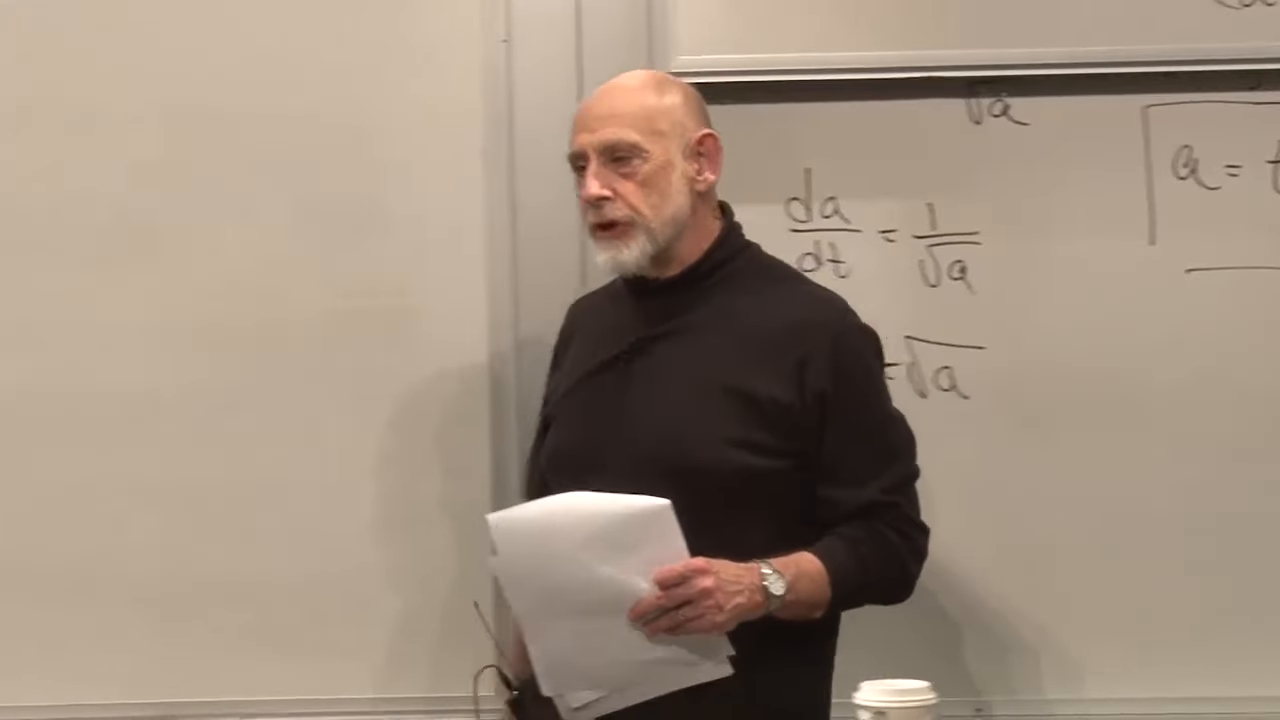
\includegraphics[width=0.68\textwidth]{lecture_02_figure_02.png}
\caption{На итоговой доске записаны \(\dot a=1/\sqrt a\) и заключённый в рамку закон при доминировании вещества \(a\propto t^{2/3}\). Промежуточные алгебраические шаги частично закрыты и приведены в уравнениях~\eqref{eq:c02-zero-energy-friedmann}--\eqref{eq:c02-matter-law}.}
\label{fig:c02-matter-recap}
\lectureframe{00:29:20.838}
\end{figure}

\begin{classroomqa}
\audiencequestion{Почему отрицательный квадратный корень был отброшен?}
\lecturerresponse{Само уравнение его не отбрасывает. Уравнение~\eqref{eq:c02-zero-energy-friedmann} фиксирует \(H^2\), а не знак \(H\). Положительный корень описывает расширение, а отрицательный — сжатие. Камень в гравитационном поле планеты может двигаться наружу или внутрь, подчиняясь одному и тому же уравнению энергии; ветвь выбирается его начальным условием. Мы выбрали ветвь расширения, потому что обсуждаем именно такую Вселенную. \lecturetimestamp{00:23:09--00:24:46}}
\end{classroomqa}

В следующей модели тёмная энергия по-прежнему будет опущена. Это сделано намеренно: сначала мы поймём более старую схему вещества и излучения, а уже потом добавим компоненту, управляющую нынешней эпохой ускоренного расширения. Тёмная материя, напротив, уже включена в член вещества, потому что нерелятивистская тёмная материя тоже разрежается как \(a^{-3}\).

\begin{classroomqa}
\audiencequestion{Разве тёмная энергия сегодня не является доминирующей компонентой?}
\lecturerresponse{Да. Развиваемая здесь история с двумя компонентами — это стандартная учебная космология времён до открытия нынешнего ускорения. Тёмная материя относится к веществу; тёмная энергия — третья компонента, которую нужно вводить отдельно. Начало со старой модели позволяет увидеть, что именно меняет каждый дополнительный член. \lecturetimestamp{00:28:02--00:28:45}}
\end{classroomqa}

\section{Восстановление константы энергии}

Выбор нулевой энергии — это специальное начальное условие. Чтобы от него отказаться, вернёмся к галактике массы \(m\) на границе однородной сферы. Пусть её сопутствующий радиус равен \(x\), так что
\begin{equation}
D=ax,
\qquad
\dot D=\dot a x.
\label{eq:c02-comoving-particle}
\end{equation}
Теорема Ньютона о сферических слоях утверждает, что на радиальное ускорение влияет только масса \(M(D)\) внутри сферы; внешние сферические оболочки не создают результирующей силы. Сохраняющаяся ньютоновская энергия галактики равна
\begin{equation}
\frac{1}{2}m\dot D^{\,2}-\frac{GM(D)m}{D}=E.
\label{eq:c02-newton-energy}
\end{equation}
Множитель \(m\) должен входить в оба члена. Его легко опустить, быстро записывая формулу на доске, но если его сохранить, становится ясно, что конечная постоянная есть энергия на единицу пробной массы.

Однородность позволяет выбрать репрезентативную галактику при \(x=1\). Тогда \(D=a\), \(\dot D=\dot a\), и для сферы имеем
\begin{equation}
V_{\rm sph}=\frac{4\pi}{3}a^3,
\qquad
M(a)=\rho_m V_{\rm sph}=\frac{4\pi}{3}\rho_m a^3.
\label{eq:c02-enclosed-mass}
\end{equation}
На доске символ \(V\) используется и для объёма, и, в боковой пометке, для радиальной скорости. Мы будем сохранять однозначные обозначения \(V_{\rm sph}\) и \(\dot D\).

\begin{figure}[ht]
\centering
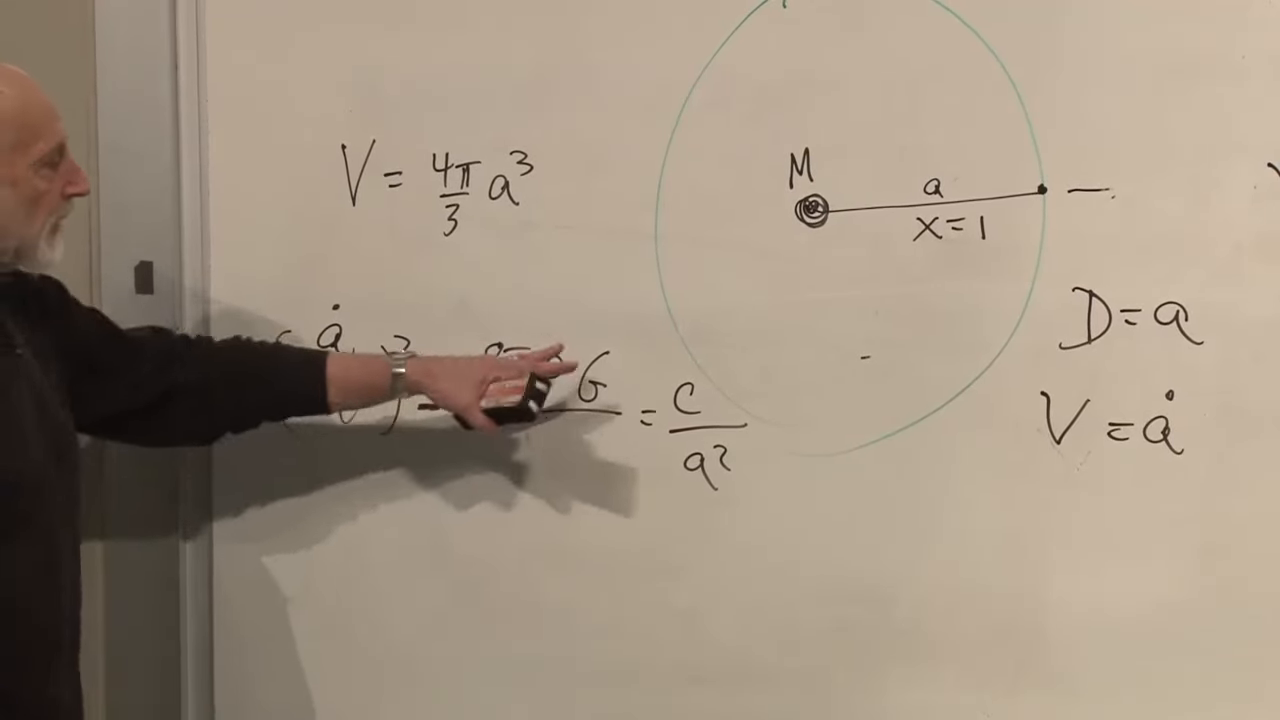
\includegraphics[width=0.86\textwidth]{lecture_02_figure_03.png}
\caption{Сфера с заключённой массой и уравнение Фридмана для ненулевой энергии. Среди видимых обозначений есть \(V_{\rm sph}=4\pi a^3/3\), центральная масса \(M\), \(x=1\), \(D=a\) и \(\dot D=\dot a\). Часть уравнения закрыта лектором и ниже восстанавливается алгебраически.}
\label{fig:c02-energy-board}
\lectureframe{00:37:59.876}
\end{figure}

\begin{figure}[ht]
\centering
\begin{tikzpicture}[scale=1.05,>=Latex]
  \draw[thick] (0,0) circle (2.6);
  \fill (0,0) circle (2.2pt) node[below left=2pt] {\(M(a)\)};
  \draw[thick,->] (0,0) -- (2.58,0);
  \fill (2.6,0) circle (2.2pt) node[right=4pt] {galaxy \(m\)};
  \node[above] at (1.30,0.04) {\(D=ax\)};
  \node[below] at (1.30,-0.04) {\(x=1\Rightarrow D=a\)};
  \draw[->,blue!60!black,thick] (2.63,0.18) -- (3.55,0.72)
    node[right] {\(\dot D=\dot a\)};
  \node at (0,-3.05) {\(M(a)=\frac{4\pi}{3}\rho_m a^3\)};
\end{tikzpicture}
\caption{Аккуратная реконструкция ньютоновской сферы при \(x=1\). Внешние оболочки взаимно сокращаются, поэтому граничная галактика реагирует только на заключённую внутри массу.}
\label{fig:c02-sphere-redraw}
\end{figure}

Подставим \(D=a\) в уравнение~\eqref{eq:c02-newton-energy}, разделим на \(m/2\) и определим постоянную
\begin{equation}
C\equiv\frac{2E}{m}.
\end{equation}
Получаем
\begin{equation}
\dot a^{\,2}-\frac{2GM(a)}{a}=C.
\label{eq:c02-energy-a}
\end{equation}
Деля на \(a^2\) и используя уравнение~\eqref{eq:c02-enclosed-mass}, находим
\begin{equation}
\left(\frac{\dot a}{a}\right)^2-
\frac{8\pi G}{3}\rho_m=\frac{C}{a^2},
\label{eq:c02-energy-form}
\end{equation}
или, эквивалентно,
\begin{equation}
\boxed{H^2=\frac{8\pi G}{3}\rho_m+\frac{C}{a^2}.}
\label{eq:c02-friedmann-C}
\end{equation}
Это первое уравнение Фридмана для вещества без давления, записанное в ньютоновской энергетической конвенции. Новый член \(a^{-2}\) хранит информацию о том, была ли начальная энергия репрезентативной галактики выше, равна или ниже энергии убегания.

Подставляя \(\rho_m=\nu_m/a^3\), удобно определить
\begin{equation}
A_m\equiv\frac{8\pi G\nu_m}{3}>0,
\end{equation}
так что
\begin{equation}
H^2=\frac{A_m}{a^3}+\frac{C}{a^2},
\qquad
\dot a^{\,2}=\frac{A_m}{a}+C.
\label{eq:c02-energy-branches}
\end{equation}
Это уравнение информативнее читать через предельные случаи, чем сразу интегрировать.

\subsection{Положительная энергия}

Если \(C>0\), то член вещества \(A_m/a^3\) доминирует при малых \(a\). Поэтому раннее расширение сохраняет закон для вещества \(a\propto t^{2/3}\). Однако при больших \(a\) в \(H^2\) доминирует член \(C/a^2\), или, эквивалентно,
\begin{equation}
\dot a^{\,2}\longrightarrow C.
\end{equation}
Расширение стремится к постоянной скорости,
\begin{equation}
a(t)\sim\sqrt C\,t.
\label{eq:c02-positive-late}
\end{equation}
Это космологический аналог броска яблока со скоростью, превышающей скорость убегания. Гравитация непрерывно уменьшает его скорость, но далеко от планеты яблоко сохраняет ненулевую асимптотическую скорость.

\subsection{Нулевая энергия}

При \(C=0\) уравнение~\eqref{eq:c02-energy-branches} дает критическое решение \(a\propto t^{2/3}\). Масштабный фактор неограниченно растет, тогда как \(\dot a\) стремится к нулю. Это в точности случай энергии убегания.

\subsection{Отрицательная энергия}

Если \(C=-|C|<0\), то
\begin{equation}
H^2=\frac{A_m}{a^3}-\frac{|C|}{a^2}
=\frac{A_m-|C|a}{a^3}.
\label{eq:c02-negative-energy}
\end{equation}
Масштабный фактор не может превысить
\begin{equation}
a_{\max}=\frac{A_m}{|C|},
\label{eq:c02-amax}
\end{equation}
потому что правая часть там обращается в нуль. Ветвь расширения достигает \(a_{\max}\) при \(\dot a=0\); ее продолжением является ветвь сжатия. В ньютоновской картине это яблоко, запущенное со скоростью меньше скорости убегания: оно поднимается, разворачивается и падает.

\begin{classroomqa}
\audiencequestion{Как модель может снова сжаться, если правая часть равна \(H^2\) и потому не может быть отрицательной?}
\lecturerresponse{Она никогда не становится отрицательной. При расширении правая часть убывает до нуля при \(a_{\max}\). Там \(H=0\). Затем решение переходит от положительного квадратного корня к отрицательному квадратному корню и проходит допустимую область обратно, с \(\dot a<0\). Заманчивое, но неверное продолжение позволило бы выражению пройти через нуль. Это невозможно: нуль — это граница, а не значение, через которое может продолжаться вещественная величина \(H\). \lecturetimestamp{00:48:43--00:53:03}}
\end{classroomqa}

Итак, три ньютоновские энергии дают три качественные истории: повторное сжатие для \(C<0\), критический случай убегания для \(C=0\) и вечное расширение с асимптотически постоянным \(\dot a\) для \(C>0\). Удивительный следующий шаг состоит в том, что общая теория относительности придает этим же случаям геометрический смысл.

\section{От энергии к кривизне}

Перенесем энергетический член в уравнении~\eqref{eq:c02-friedmann-C} на геометрическую сторону и определим
\begin{equation}
k\equiv-C.
\label{eq:c02-k-definition}
\end{equation}
Тогда
\begin{equation}
\boxed{H^2+\frac{k}{a^2}=\frac{8\pi G}{3}\rho.}
\label{eq:c02-friedmann-k}
\end{equation}
На доске попеременно используются обозначения \(C\), \(K\) и \(\kappa\), а при переносе члена через знак равенства поглощается знак. Уравнение~\eqref{eq:c02-k-definition} фиксирует наше соглашение о знаках: положительной ньютоновской энергии соответствует \(k<0\), нулевой энергии — \(k=0\), а отрицательной ньютоновской энергии — \(k>0\).

\begin{figure}[ht]
\centering
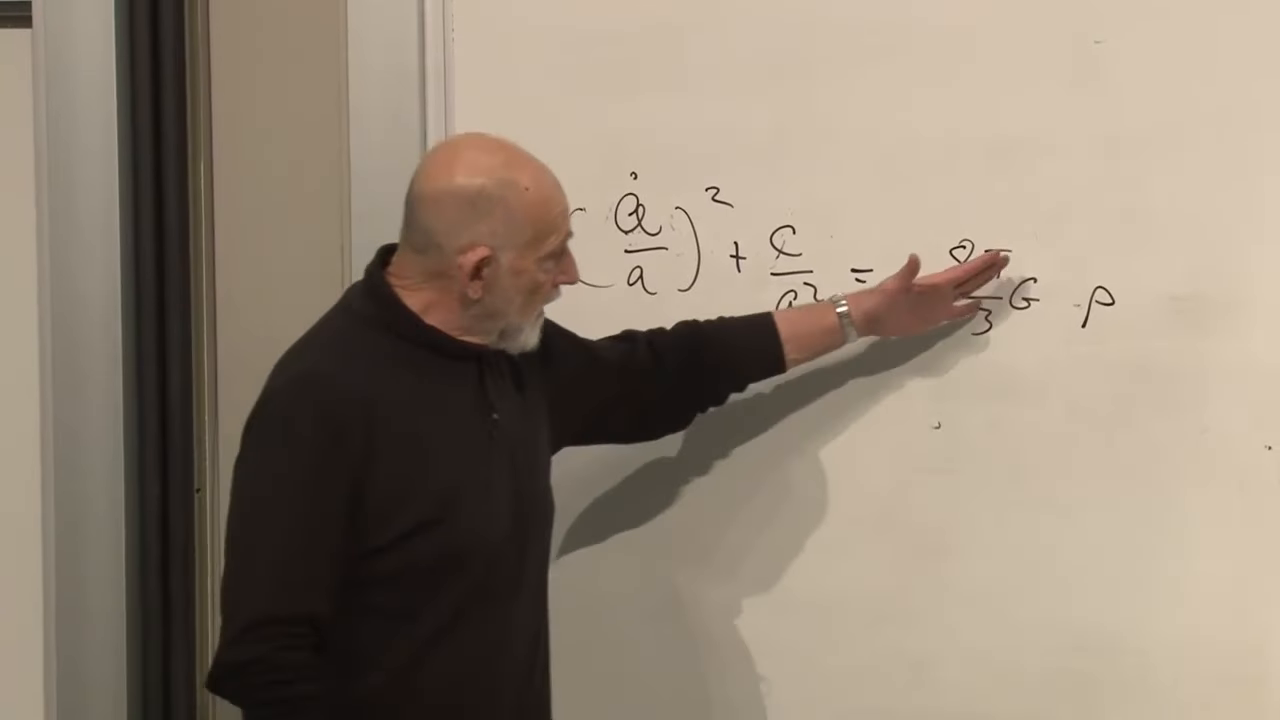
\includegraphics[width=0.76\textwidth]{lecture_02_figure_04.png}
\caption{Уравнение Фридмана, записанное так, что геометрия стоит слева, а источник — справа. Рамка поддерживает это концептуальное разделение; полное тензорное уравнение Эйнштейна в ней не показано.}
\label{fig:c02-geometry-source}
\lectureframe{00:55:22.810}
\end{figure}

Такое расположение — уменьшенная версия уравнения Эйнштейна. Левая часть описывает геометрию: расширение через \(H\) и пространственную кривизну через \(k/a^2\). Правая часть описывает материальный источник. В ньютоновской механике этим источником была плотность массы. В теории относительности это энергия и импульс, полностью описываемые тензором энергии-импульса. Для однородной и изотропной Вселенной первое уравнение Фридмана зависит от полной плотности энергии \(\rho\).

Если сохранять обычные единицы, плотность массы вносит вклад через свою энергию покоя \(\rho_{\rm mass}c^2\). Отныне положим \(c=1\), так что масса и энергия выражаются в одних и тех же единицах. Тогда символ \(\rho\) может включать массу покоя, кинетическую энергию, излучение и любую другую однородную компоненту энергии.

\begin{figure}[ht]
\centering
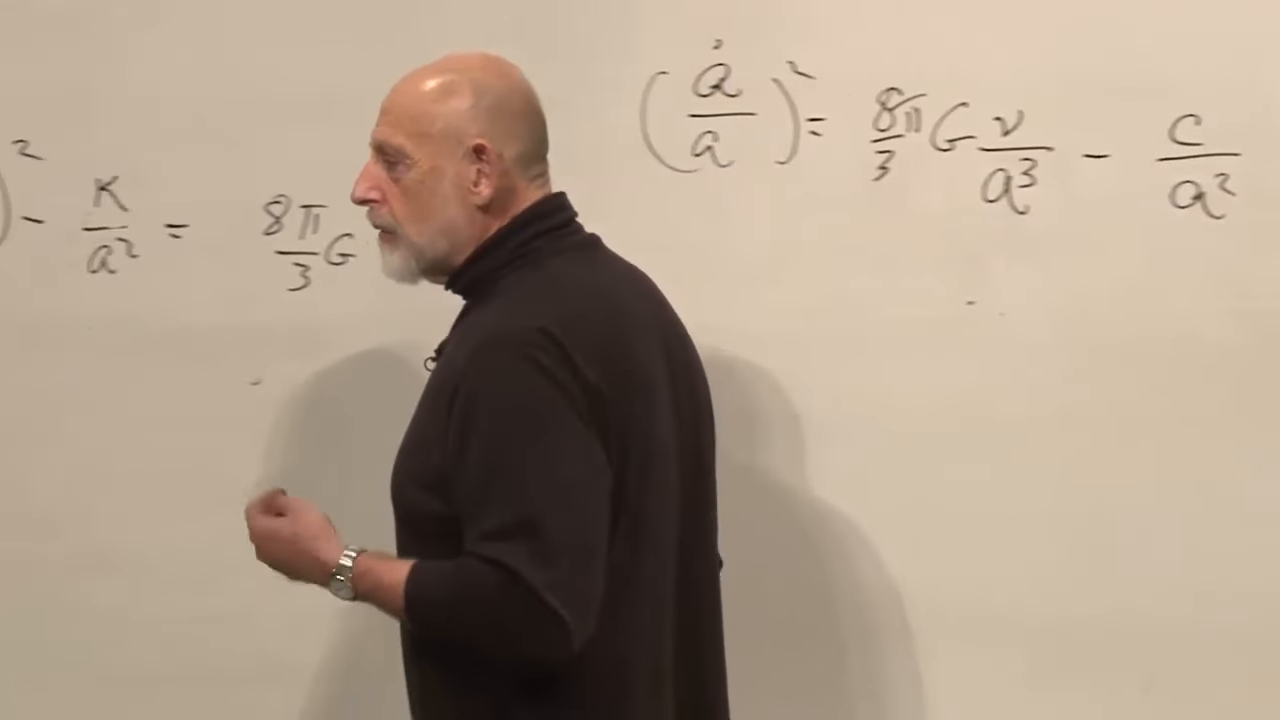
\includegraphics[width=0.88\textwidth]{lecture_02_figure_05.png}
\caption{Две записанные на доске формы уравнения Фридмана рядом: форма с кривизной, использующая \(\rho\), и форма с веществом, полученная после подстановки \(\rho_m=\nu_m/a^3\). Обозначения на доске меняются; уравнение~\eqref{eq:c02-k-definition} сохраняет используемое здесь соглашение о знаках.}
\label{fig:c02-curvature-comparison}
\lectureframe{00:57:52.659}
\end{figure}

Геометрическая интерпретация глобальна. В релятивистской модели \(k=0\) описывает плоские пространственные срезы, \(k>0\) — сферические срезы положительной кривизны, а \(k<0\) — гиперболические срезы отрицательной кривизны. Ньютоновский вывод воспроизвел то же уравнение эволюции, не располагая этими глобальными геометриями. Поэтому его ненулевая постоянная энергии — замечательно точный аналог кривизны, но не вывод самого искривленного пространства.

\begin{classroomqa}
\audiencequestion{Как ньютоновская механика и общая теория относительности могут давать одно и то же уравнение расширения, если их геометрии различны?}
\lecturerresponse{Общая теория относительности включает и плоский случай, а локально всякая гладкая геометрия приблизительно плоска. Еще более замечательно то, что ньютоновская постоянная энергии входит в уравнение эволюции точно в то место, которое в релятивистской теории занимает пространственная кривизна. Динамическая формула совпадает, а глобальная интерпретация — нет: евклидово ньютоновское пространство не превратилось тайно в сферу или гиперболическое пространство. Все три геометрии придется построить в рамках общей теории относительности. \lecturetimestamp{01:20:59--01:24:20}}
\end{classroomqa}

\section{Излучение в расширяющемся ящике}

Теперь мы изменим содержимое Вселенной. Рассмотрим один сопутствующий единичный куб. Его физический объем равен \(a^3\). Для нерелятивистского вещества число частиц в этом ящике фиксировано, и энергия покоя каждой частицы приблизительно постоянна, что дает \(\rho_m\propto a^{-3}\). Для излучения есть еще один эффект: по мере расширения Вселенной каждый фотон теряет энергию.

Фотон с длиной волны \(\lambda\) имеет энергию
\begin{equation}
E_\gamma=\frac{hc}{\lambda},
\qquad
E_\gamma\propto\lambda^{-1}.
\label{eq:c02-photon-energy}
\end{equation}
При однородном расширении свободно распространяющаяся длина волны растягивается пропорционально масштабному фактору:
\begin{equation}
\frac{\lambda(t_2)}{\lambda(t_1)}
=\frac{a(t_2)}{a(t_1)},
\qquad
\lambda\propto a.
\label{eq:c02-redshift}
\end{equation}
Это космологическое красное смещение. Из него следует
\begin{equation}
E_\gamma\propto a^{-1}.
\label{eq:c02-photon-redshift}
\end{equation}
Если число фотонов в сопутствующем ящике сохраняется, полная энергия излучения в нем убывает как \(a^{-1}\). Деление на физический объем \(a^3\) дает
\begin{equation}
\boxed{\rho_r(a)=\frac{\nu_r}{a^4}.}
\label{eq:c02-radiation-density}
\end{equation}
Здесь \(\nu_r\) — постоянный коэффициент плотности свободно распространяющегося излучения. У излучения на одну обратную степень \(a\) больше, чем у вещества: три степени возникают из-за пространственного разбавления и одна — из красного смещения каждого фотона.

Аналогия с гитарной струной дает полезную интуицию. Мода, укладывающаяся на струне, имеет целое число полуволн. Если струну медленно удлинять, это целое число не может изменяться непрерывно; вместо этого длина волны подстраивается под новую длину. Аналогично, для волны на медленно расширяющемся кольце число узлов является адиабатическим инвариантом, поэтому ее длина волны следует за длиной окружности. Произвольную волну можно разложить по таким модам.

Это не заменяет решения уравнений Максвелла в расширяющемся пространстве-времени. Это та обоснованная интуиция, которая стоит за уравнением~\eqref{eq:c02-redshift}: медленное геометрическое расширение изменяет физическую длину волны, сохраняя метку моды.

\begin{classroomqa}
\audiencequestion{Требует ли этот аргумент проводящего или отражающего ящика? Что происходит в пустом расширяющемся пространстве без физических стен?}
\lecturerresponse{Стены — это средство учета, а не утверждение, что Вселенная заключена в проводящую оболочку. Полное доказательство следует из распространения волн в расширяющейся метрике. Для настоящего аргумента мы используем наблюдаемый и выведенный из общей теории относительности факт, что свободно распространяющиеся длины волн масштабируются как \(a\). Ящик помогает считать фотоны и физический объем; он не вызывает космологического красного смещения. \lecturetimestamp{01:02:21--01:04:37}}
\end{classroomqa}

\begin{classroomqa}
\audiencequestion{Почему длина волны должна следовать за сеткой, а не сохранять фиксированную физическую длину?}
\lecturerresponse{Рассмотрим моду на кольце, длина окружности которого адиабатически меняется. Ее целочисленное число узлов не может непрерывно изменяться, поэтому допустимая длина волны должна изменяться вместе с кольцом. Разложение произвольной волны в Фурье-моды приводит к тому же выводу для каждой моды по отдельности. Это дает нужную адиабатическую интуицию; точное утверждение относится к теории поля в искривленном пространстве-времени. \lecturetimestamp{01:34:18--01:38:33}}
\end{classroomqa}

\subsection{Решение при доминировании излучения}

Временно опустив кривизну, подставим уравнение~\eqref{eq:c02-radiation-density} в уравнение Фридмана:
\begin{equation}
H^2=\frac{8\pi G\nu_r}{3a^4}
\equiv\frac{A_r}{a^4},
\qquad A_r>0.
\label{eq:c02-radiation-friedmann}
\end{equation}
На ветви расширения
\begin{equation}
\frac{\dot a}{a}=\frac{\sqrt{A_r}}{a^2},
\qquad
\dot a=\frac{\sqrt{A_r}}{a}.
\end{equation}
Следовательно,
\begin{equation}
a\,da=\sqrt{A_r}\,dt,
\qquad
\frac{a^2}{2}=\sqrt{A_r}(t-t_B),
\end{equation}
и
\begin{equation}
\boxed{a(t)\propto(t-t_B)^{1/2}.}
\label{eq:c02-radiation-law}
\end{equation}
Различие между показателями степени \(1/2\) и \(2/3\) визуально невелико, но физически решающе. Скорость расширения, температура, замораживание реакций и размер горизонта в ранней Вселенной — все они зависят от того, какая компонента доминирует.

\section{Вселенная из вещества и излучения}

Для вещества и излучения, сохраняющихся по отдельности, их плотности складываются:
\begin{equation}
\rho(a)=\rho_m(a)+\rho_r(a).
\end{equation}
Пренебрегая кривизной в этом сравнении,
\begin{equation}
\boxed{H^2=\frac{C_m}{a^3}+\frac{C_r}{a^4},}
\label{eq:c02-mixed-friedmann}
\end{equation}
где \(C_m,C_r>0\). На доске два коэффициента сначала обозначены как \(C_1\) и \(C\); второе обозначение затем устно исправляется на другую константу. Обозначение в уравнении~\eqref{eq:c02-mixed-friedmann} делает это исправление явным.

\begin{figure}[ht]
\centering
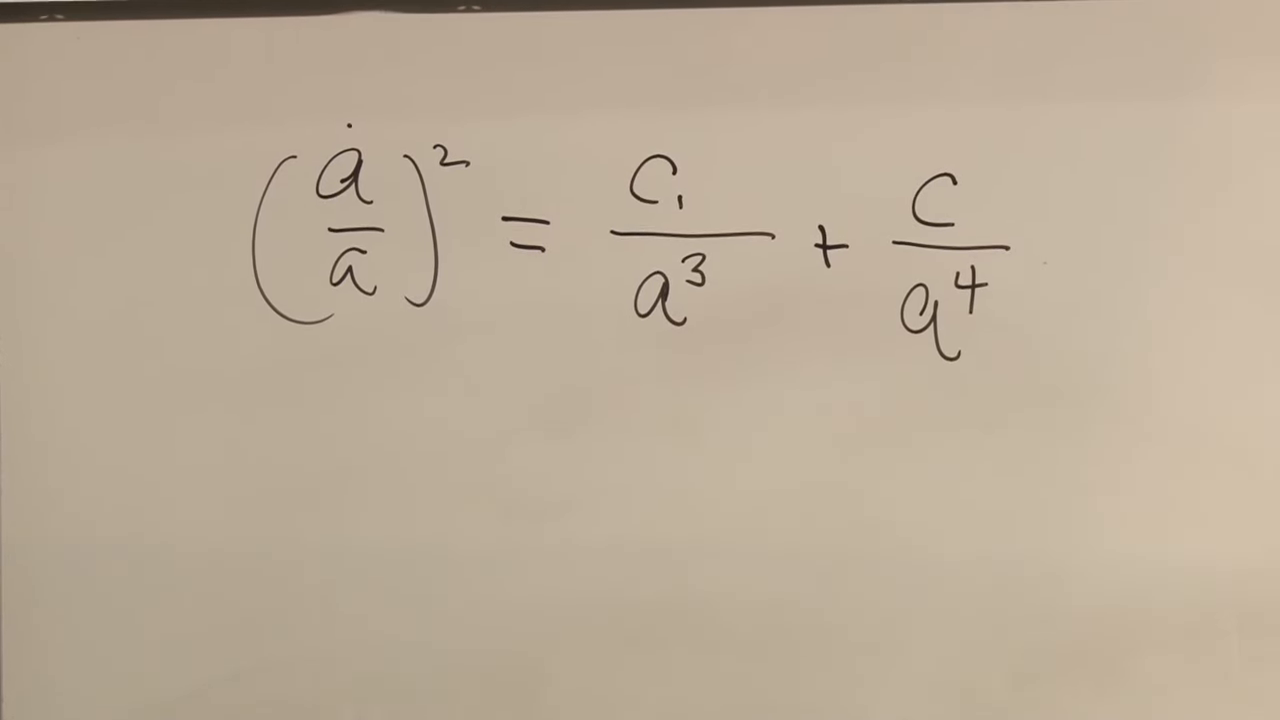
\includegraphics[width=0.74\textwidth]{lecture_02_figure_06.png}
\caption{Смешанное уравнение для вещества и излучения на доске. Записанный второй коэффициент затем исправляется на константу, относящуюся именно к излучению и обозначенную \(C_r\) в уравнении~\eqref{eq:c02-mixed-friedmann}.}
\label{fig:c02-mixed-board}
\lectureframe{01:11:37.997}
\end{figure}

При малых \(a\) доминирует член излучения, потому что \(a^{-4}\) растет быстрее, чем \(a^{-3}\):
\begin{equation}
a\ll a_{\rm eq}
\quad\Longrightarrow\quad
H^2\simeq\frac{C_r}{a^4},
\qquad
a(t)\propto t^{1/2}.
\end{equation}
При больших \(a\) доминирует вещество:
\begin{equation}
a\gg a_{\rm eq}
\quad\Longrightarrow\quad
H^2\simeq\frac{C_m}{a^3},
\qquad
a(t)\propto t^{2/3}.
\end{equation}
Значение масштабного фактора при равенстве сразу получается из приравнивания двух членов:
\begin{equation}
a_{\rm eq}=\frac{C_r}{C_m}.
\label{eq:c02-equality-scale}
\end{equation}
Это равенство — не то же самое событие, что и расцепление фотонов. Равенство означает момент, когда две плотности энергии совпадают; расцепление — момент, когда взаимодействия перестают удерживать вещество и излучение в тепловом контакте.

Сектор излучения включает фотоны и любые виды частиц, движущиеся ультрарелятивистски. Очень лёгкие нейтрино ведут себя так при достаточно высокой температуре, и фон гравитонов масштабировался бы таким же образом. Как только массивный вид частиц становится нерелятивистским, его доминирующий вклад от массы покоя начинает масштабироваться как вещество. Холодная тёмная материя относится к \(C_m/a^3\), а не к члену излучения.

\begin{classroomqa}
\classquestion{Какой член в уравнении~\eqref{eq:c02-mixed-friedmann} доминирует сначала, а какой — позже?}
\lecturerresponse{При малых \(a\) член \(a^{-4}\) превосходит \(a^{-3}\), поэтому на ранней стадии расширение контролируется излучением и получается \(a\propto t^{1/2}\). По мере роста \(a\) отношение излучения к веществу падает как \(1/a\); тогда расширение контролируется веществом и получается \(a\propto t^{2/3}\). \lecturetimestamp{01:11:46--01:13:38}}
\end{classroomqa}

\begin{classroomqa}
\audiencequestion{Предполагается ли, что относительные количества вещества и излучения постоянны?}
\lecturerresponse{Их плотности не постоянны, но коэффициенты \(C_m\) и \(C_r\) можно считать постоянными после того, как компоненты перестают эффективно обмениваться энергией и рождением или аннигиляцией частиц можно пренебречь. Тогда для вещества сохраняется сопутствующая масса покоя, а для свободного излучения — сопутствующее число фотонов, причём красное смещение даёт ему дополнительный множитель \(a^{-1}\). В эпохи сильного взаимодействия или аннигиляции видов частиц этот учёт нужно уточнять. \lecturetimestamp{01:13:39--01:14:53}}
\end{classroomqa}

\begin{classroomqa}
\audiencequestion{Когда вещество и излучение перестали сильно взаимодействовать?}
\lecturerresponse{Грубый ответ по порядку величины — \(10^5\) лет для развязки фотонов с обычным веществом. Точная история рекомбинации вычисляется позже, и её не следует путать с эпохой равенства вещества--излучения. Здесь нужно лишь то, что после развязки эти две компоненты можно отслеживать приблизительно по отдельности. \lecturetimestamp{01:27:29--01:27:46}}
\end{classroomqa}

\begin{classroomqa}
\audiencequestion{Как мы можем знать, что ранняя эпоха \(a\propto t^{1/2}\) имела место до того, как появились галактики, по которым можно прослеживать расширение?}
\lecturerresponse{Мы выводим историю расширения из тех физических следов, которые оно оставляет. Первичный нуклеосинтез зависит от раннего соперничества между скоростями реакций и \(H(t)\); микроволновой фон фиксирует более позднее тепловое состояние и возмущения. Наблюдения галактик дают более прямые сведения о поведении в эпоху вещества, тогда как эпоха излучения реконструируется по этим свидетельствам ранней Вселенной. \lecturetimestamp{01:27:46--01:30:10}}
\end{classroomqa}

Модель вещества и излучения заведомо неполна. Это классическая схема, в которой Вселенная переходит от доминирования излучения к доминированию вещества. Нынешнее ускоренное расширение требует другого источника — тёмной энергии, которая добавит качественно иной член.

\section{Куда девается энергия при красном смещении}

Убывание, задаваемое соотношением \(E_\gamma\propto a^{-1}\), ставит неизбежный вопрос: куда делась энергия фотонов? В буквальном расширяющемся ящике с отражающими стенками излучение оказывает давление и совершает работу над стенками. Термодинамическое утверждение таково:
\begin{equation}
dE=-p\,dV.
\label{eq:c02-pdv}
\end{equation}
При увеличении \(V\) энергия излучения уменьшается. Потерянная энергия может перейти в кинетическую энергию, энергию деформации или тепло в том, что движет стенки.

У сопутствующего ящика нет материальных стенок. Это воображаемая граница, движущаяся вместе со средним расширением. Фотоны пересекают её, но в однородной ванне излучения статистический поток, входящий внутрь, уравновешивает поток, выходящий наружу. Такой ящик остаётся корректным учётным объёмом, хотя контейнером он не является. Закон работы давления по-прежнему описывает, как эволюционирует энергия в сопутствующем объёме.

Для излучения \(p=\rho/3\), и \(E=\rho V\). Тогда уравнение~\eqref{eq:c02-pdv} даёт
\begin{align}
d(\rho V)&=-\frac{\rho}{3}\,dV,\\
V\,d\rho&=-\frac{4}{3}\rho\,dV,\\
\frac{d\rho}{\rho}&=-\frac{4}{3}\frac{dV}{V}.
\end{align}
Поскольку \(V\propto a^3\), интегрирование даёт \(\rho\propto a^{-4}\), что согласуется с аргументом через длину волны. Этот термодинамический вывод также ясно показывает, что уменьшается энергия каждого фотона, а не только численная плотность.

\begin{classroomqa}
\audiencequestion{Куда девается энергия фотонов при красном смещении? Сохраняется ли полная энергия Вселенной?}
\lecturerresponse{При наличии реальных стенок излучение совершает над ними работу, так что перенос энергии описывается обычным механическим балансом. Для Вселенной в целом вопрос тоньше. Глобальное сохранение энергии обычно следует из симметрии относительно сдвига по времени, но расширяющееся пространство-время, вообще говоря, не инвариантно относительно трансляции по времени и не обязано обладать единственной сохраняющейся полной энергией. Можно построить полезные ньютоновские аналогии, включающие энергию расширения, но определённое глобальное утверждение требует общей теории относительности. Обе точки зрения здесь полезны, но из ньютоновской модели не следует никакого окончательного глобального вывода. \lecturetimestamp{01:16:51--01:20:58}}
\end{classroomqa}

\begin{classroomqa}
\audiencequestion{Если сопутствующий ящик воображаемый и фотоны пересекают его границу, как картина с работой давления всё же может быть полезной?}
\lecturerresponse{Недостающий учёт обеспечивает однородность. В среднем каждый фотон, покидающий один сопутствующий объём, статистически заменяется фотоном, входящим из соседнего. Локальные потоки в среднем компенсируют друг друга, тогда как физический объём и длины волн меняются. Отражающий ящик делает механизм работы наглядным; сопутствующий ящик несёт тот же усреднённый закон сохранения без буквальных стенок. \lecturetimestamp{01:24:22--01:27:28}}
\end{classroomqa}

\begin{classroomqa}
\audiencequestion{Расширение лишь уменьшает плотность фотонов или оно уменьшает энергию каждого фотона?}
\lecturerresponse{Происходит и то и другое. Число фотонов в единице физического объёма падает как \(a^{-3}\), а космологическое красное смещение уменьшает энергию каждого фотона ещё на множитель \(a^{-1}\). Это радиационный аналог адиабатического охлаждения. Обычный газ тоже охлаждается, совершая работу при медленном расширении, хотя внезапное свободное расширение — иной термодинамический процесс. \lecturetimestamp{01:42:30--01:45:55}}
\end{classroomqa}

\section{Рецессия, горизонты и пределы модели}

Закон Хаббла приписывает объекту на собственном расстоянии \(D\) на выбранном срезе космического времени скорость рецессии
\begin{equation}
v_{\rm rec}=HD
\label{eq:c02-recession}
\end{equation}
При достаточно больших \(D\) уравнение~\eqref{eq:c02-recession} может давать значение больше \(c\). Это не нарушает специальную теорию относительности, потому что \(v_{\rm rec}\) — не скорость близкого объекта, измеренная в одной локальной инерциальной системе отсчёта. Оно сравнивает далеко разнесённые сопутствующие мировые линии в меняющейся геометрии. Каждый локальный наблюдатель по-прежнему измеряет свет со скоростью \(c\), и ни один локальный материальный объект не обгоняет другой быстрее света.

\begin{classroomqa}
\audiencequestion{Может ли достаточно далёкая галактика удаляться быстрее света?}
\lecturerresponse{Да, её космологическая скорость рецессии \(HD\) может превышать \(c\). При этом ни один локальный объект не обгоняет соседнего наблюдателя быстрее света, и этот результат нельзя использовать для сверхсветовой передачи сигналов. Это утверждение об изменяющемся собственном расстоянии между далёкими сопутствующими мировыми линиями, а не об обычной специальнорелятивистской скорости, измеренной в одном событии. \lecturetimestamp{01:30:17--01:32:13}}
\end{classroomqa}

Сверхсветовая рецессия сама по себе не решает, достигнет ли нас когда-нибудь свет, испущенный сейчас. Это вопрос о всей будущей истории расширения. В замедляющейся модели с доминированием вещества области, которые сейчас удаляются быстрее света, позднее могут стать наблюдаемыми, потому что соответствующий горизонт эволюционирует. Если ускоренное расширение сохранится, горизонт событий может навсегда скрыть достаточно далёкие события.

\begin{classroomqa}
\audiencequestion{Исчезают ли галактики, как только их скорость рецессии превышает скорость света?}
\lecturerresponse{Не так просто. Пересечение хаббловского радиуса и настоящий горизонт событий — разные понятия. В замедляющейся модели свет из области, которая сейчас удаляется сверхсветовым образом, всё ещё может дойти до нас позже. Устойчивое доминирование тёмной энергии меняет глобальную причинную структуру и может создать предельный горизонт. Чтобы решить, какие сигналы приходят, нужна геометрия пространства-времени, а не мгновенный снимок \(HD\). \lecturetimestamp{01:32:14--01:34:18}}
\end{classroomqa}

Язык специальной теории относительности тоже может вводить в заблуждение, если применять его глобально. Инвариантная масса покоя частицы не увеличивается со скоростью. Её энергия и импульс зависят от локальной системы отсчёта наблюдателя. Массивные частицы нельзя ускорить через порог локальной скорости света, но рецессия далёкой сопутствующей галактики — не её прохождение через одну локальную систему отсчёта.

\begin{classroomqa}
\audiencequestion{Приобретает ли быстро удаляющаяся галактика большую релятивистскую массу?}
\lecturerresponse{Яснее не пользоваться термином ``релятивистская масса''. Галактика имеет инвариантную массу покоя, тогда как её энергия и импульс зависят от системы отсчёта. Более того, скорость рецессии, приписываемая на космологических расстояниях, не является локальной скоростью, входящей в специальнорелятивистскую формулу. Эти понятия согласуются лишь после того, как далёкие события сопоставлены с помощью метрики пространства-времени. \lecturetimestamp{01:38:34--01:40:05}}
\end{classroomqa}

\begin{classroomqa}
\audiencequestion{Что происходит с осями времени и пространства, когда скорость удаления далёкого объекта сверхсветовая?}
\lecturerresponse{Не существует единой глобальной лоренцевой системы отсчёта, чьи наклонённые оси позволяли бы решить этот вопрос. Специальная теория относительности сравнивает инерциальные системы отсчёта в плоском пространстве-времени; космология требует метрики, которая связывает локальные системы отсчёта в протяжённом искривлённом пространстве-времени. Ньютоновские рассуждения остаются надёжными в малой области, но к глобальному построению можно перейти лишь в общей теории относительности. \lecturetimestamp{01:40:07--01:42:30}}
\end{classroomqa}

Ньютоновское сохранение энергии привело к правильному уравнению для масштабного фактора в случае вещества и даже предвосхитило член кривизны. Волновая механика и термодинамика дают зависимость для излучения. Однако пространственная геометрия, глобальная энергия и горизонты не являются локальными ньютоновскими вопросами; они требуют метрического описания, которое следует далее.

\section{Вещество, излучение и кривизна}

Критическое решение для модели, содержащей только вещество, подчиняется
\begin{equation}
\rho_m\propto a^{-3},
\qquad
a(t)\propto t^{2/3}.
\end{equation}
Если восстановить ньютоновскую энергию на единицу массы, получаем
\begin{equation}
H^2=\frac{8\pi G}{3}\rho_m+\frac{C}{a^2}.
\end{equation}
Положительное \(C\) приводит к вечному расширению с \(a\sim t\) на поздних стадиях, \(C=0\) соответствует критическому убеганию, а отрицательное \(C\) даёт максимальный масштабный фактор, за которым следует повторный коллапс. Определение \(k=-C\) помещает тот же член в геометрическую часть релятивистского уравнения Фридмана.

Излучение отличается от вещества тем, что расширение изменяет и численную плотность, и энергию каждого кванта:
\begin{equation}
\begin{aligned}
\lambda&\propto a,
&\qquad E_\gamma&\propto a^{-1},\\
\rho_r&\propto a^{-4},
& a(t)&\propto t^{1/2}.
\end{aligned}
\end{equation}
Поэтому двухкомпонентное уравнение
\begin{equation}
H^2=\frac{C_m}{a^3}+\frac{C_r}{a^4}
\end{equation}
описывает раннюю Вселенную с доминированием излучения, за которой следует эпоха доминирования вещества. Тёмная энергия, пространственная геометрия и причинная структура горизонтов остаются вне этой модели, именно там, где ньютоновское приближение подсказывает передать задачу общей теории относительности.